%%% LaTeX-Vorlage Version 1.8 %%%

% Grundlegende Dokumenteneigenschaften gemäß DHBW-Vorgaben
\documentclass[a4paper,fontsize=11pt,oneside,parskip=half,headings=normal]{scrreprt} 
% \usepackage{showframe} % nur für Kontrolle der Ränder 

%%% Präambel einbinden (mit Festlegungen gemäß DHBW-Vorgaben) %%%
%%% Präambel %%%
% hier sollten keine Änderungen erforderlich sein
%
\usepackage[utf8]{inputenc}   % Zeichencodierung UTF-8 für Eingabe-Dateien
\usepackage[T1]{fontenc}      % Darstellung von Umlauten im PDF

\usepackage{listings}         % für Einbindung von Code-Listings
\lstset{numbers=left,numberstyle=\tiny,numbersep=5pt,texcl=true}
\lstset{literate=             % erlaubt Sonderzeichen in Code-Listings 
{Ö}{{\"O}}1
{Ä}{{\"A}}1
{Ü}{{\"U}}1
{ß}{{\ss}}2
{ü}{{\"u}}1
{ä}{{\"a}}1
{ö}{{\"o}}1
{€}{{\euro}}1
}

\usepackage[
  inner=35mm,outer=15mm,top=25mm,
  bottom=20mm,foot=12mm,includefoot
]{geometry}                 % Einstellungen für Ränder

%\usepackage[ngerman]{babel} % Spracheinstellungen Deutsch
%\usepackage[babel,german=quotes]{csquotes} % deutsche Anf.zeichen
\usepackage[english]{babel} % Spracheinstellungen Englisch
\usepackage[babel,english=british]{csquotes} % englische Anf.zeichen
\usepackage{enumerate}      % anpassbare Nummerier./Aufz.
\usepackage{enumitem}
\usepackage{graphicx}       % Einbinden von Grafiken
\usepackage[onehalfspacing]{setspace} % anderthalbzeilig

\usepackage{blindtext}      % Textgenerierung für Testzwecke
\usepackage{color}          % Verwendung von Farbe 
\usepackage{float}
\usepackage{acronym}        % für ein Abkürzungsverzeichnis
\usepackage{comment}
\usepackage[                % Biblatex
  backend=biber,
  bibstyle=_dhbw_authoryear,maxbibnames=99,
  citestyle=authoryear,     
  uniquename=true, useprefix=true,
  bibencoding=utf8]{biblatex}
%kein Punkt am Ende bei \footcite
%http://www.golatex.de/footcite-ohne-punkt-am-schluss-t4865.html
\renewcommand{\bibfootnotewrapper}[1]{\bibsentence#1}


%Reihenfolge der Autorennamen
%   
% http://golatex.de/viewtopic,p,80448.html#80448
% Argumente: siehe http://texwelt.de/blog/modifizieren-eines-biblatex-stils/
\DeclareNameFormat{sortname}{% Bibliographie
  \ifnum\value{uniquename}=0 % Normalfall
    \ifuseprefix%
      {%
         \usebibmacro{name:family-given}
           {\namepartfamily}
           {\namepartgiveni}
           {\namepartprefix}
           {\namepartsuffixi}%
       }
      {%
         \usebibmacro{name:family-given}
           {\namepartfamily}
           {\namepartgiveni}
           {\namepartprefixi}
           {\namepartsuffixi}%
       }%
  \fi
  \ifnum\value{uniquename}=1% falls nicht eindeutig, abgek. Vorname 
      {%
         \usebibmacro{name:family-given}
           {\namepartfamily}
           {\namepartgiveni}
           {\namepartprefix}
           {\namepartsuffix}%
       }%
  \fi
  \ifnum\value{uniquename}=2% falls nicht eindeutig, ganzer Vorname 
      {%
         \usebibmacro{name:family-given}
           {\namepartfamily}
           {\namepartgiven}
           {\namepartprefix}
           {\namepartsuffix}%
       }%
  \fi   
  \usebibmacro{name:andothers}}

\DeclareNameFormat{labelname}{% für Zitate
  \ifnum\value{uniquename}=0 % Normalfall
    \ifuseprefix%
      {%
         \usebibmacro{name:family-given}
           {\namepartfamily}
           {\empty}
           {\namepartprefix}
           {\namepartsuffixi}%
       }
      {%
         \usebibmacro{name:family-given}
           {\namepartfamily}
           {\empty}
           {\namepartprefixi}
           {\namepartsuffixi}%
       }%
  \fi
  \ifnum\value{uniquename}=1% falls nicht eindeutig, abgek. Vorname 
      {%
         \usebibmacro{name:family-given}
           {\namepartfamily}
           {\namepartgiveni}
           {\namepartprefix}
           {\namepartsuffix}%
       }%
  \fi
  \ifnum\value{uniquename}=2% falls nicht eindeutig, ganzer Vorname 
      {%
         \usebibmacro{name:family-given}
           {\namepartfamily}
           {\namepartgiven}
           {\namepartprefix}
           {\namepartsuffix}%
       }%
  \fi   
  \usebibmacro{name:andothers}}
      
  
\DeclareFieldFormat{extrayear}{% = the 'a' in 'Jones 1995a'
  \iffieldnums{labelyear}
    {\mknumalph{#1}}
    {\mknumalph{#1}}}        

\renewcommand*{\multinamedelim}{\addslash}
\renewcommand*{\finalnamedelim}{\addslash}
\renewcommand*{\multilistdelim}{\addslash}
\renewcommand*{\finallistdelim}{\addslash}

\renewcommand{\nameyeardelim}{~}

% urverzeichnis: Doppelpunkt zwischen Name (Jahr): Rest 
% http://de.comp.text.tex.narkive.com/Tn1HUIXB/biblatex-authoryear-und-doppelpunkt
\renewcommand{\labelnamepunct}{\addcolon\addspace}

% damit die Darstellung für Vollzitate von Primärquellen in 
% Fußnoten später auf "nicht fett" geändert werden kann 
% (nur für Zitate von Sekundärliteratur relevant)
\newcommand{\textfett}[1]{\textbf{#1}}

% für Zitate von Sekundärliteratur:
\newcommand{\footcitePrimaerSekundaer}[4]{%
  \renewcommand{\textfett}[1]{##1}%
  \footnote{\fullcite[#2]{#1}, zitiert nach \cite[#4]{#3}}%  
  \renewcommand{\textfett}[1]{\textbf{##1}}%
}

% Im Literaturverzeichnis: Autor (Jahr) fett
\renewbibmacro*{author}{%
  \ifboolexpr{%
    test \ifuseauthor%
    and
    not test {\ifnameundef{author}}
  }
    {\usebibmacro{bbx:dashcheck}
       {\bibnamedash}
       {\usebibmacro{bbx:savehash}%
        \textfett{\printnames{author}}%
        \iffieldundef{authortype}
          {\setunit{\addspace}}
          {\setunit{\addcomma\space}}}%
     \iffieldundef{authortype}
       {}
       {\usebibmacro{authorstrg}%
        \setunit{\addspace}}}%
    {\global\undef\bbx@lasthash
     \usebibmacro{labeltitle}%
     \setunit*{\addspace}}%
  \textfett{\usebibmacro{date+extrayear}}}

% Sonderfall: Quelle ohne Autor, aber mit Herausgeber
% Name des Herausgebers wird fett gedruckt
\renewbibmacro*{bbx:editor}[1]{%
  \ifboolexpr{%
    test \ifuseeditor%
    and
    not test {\ifnameundef{editor}}
  }
    {\usebibmacro{bbx:dashcheck}
       {\bibnamedash}
       {\textfett{\printnames{editor}}%
        \setunit{\addcomma\space}%
        \usebibmacro{bbx:savehash}}%
     \usebibmacro{#1}%
     \clearname{editor}%
     \setunit{\addspace}}%
    {\global\undef\bbx@lasthash
     \usebibmacro{labeltitle}%
     \setunit*{\addspace}}%
  \textfett{\usebibmacro{date+extrayear}}}

% Anpassungen für deutsche Sprache
\DefineBibliographyStrings{ngerman}{%
	nodate = {{o.J.}},
	urlseen = {{Abruf:}},
	ibidem = {{ebenda}}
}

% keine Anführungszeichen beim Titel im Literaturverzeichnis
\DeclareFieldFormat[article,book,inbook,inproceedings,manual,misc,phdthesis,thesis,online,report]{title}{#1\isdot}

\newcommand{\literaturverzeichnis}{%
% nur Literaturverzeichnis
% (als eigenes Kapitel)
\phantomsection
\addcontentsline{toc}{chapter}{List of literature}
\spezialkopfzeile{List of literature}
\defbibheading{lit}{\chapter*{List of literature}}
\label{chapter:quellen}
\printbibliography[heading=lit,notkeyword=ausblenden]
}

% Anpassungen für englische Sprache
\DefineBibliographyStrings{english}{
	nodate = {{w.y.}},
	urlseen = {{retrieval:}},
	andothers = {{inter alia}}
} % mit DHBW-spezifischen Einstellungen

% If you want to break on URL numbers
\setcounter{biburlnumpenalty}{9000}
% If you want to break on URL lower case letters
\setcounter{biburllcpenalty}{9000}
% If you want to break on URL UPPER CASE letters
\setcounter{biburlucpenalty}{9000}

%\usepackage{xurl}
%\PassOptionsToPackage{hyphens}{url}
\usepackage[hidelinks]{hyperref}
\def\UrlBreaks{\do\/\do-}



\def\hyphenateAndTtWholeString #1{\xHyphenate#1$\wholeString\unskip}

\def\xHyphenate#1#2\wholeString {\if#1$%
	\else\transform{#1}%
	\takeTheRest#2\ofTheString\fi}

\def\takeTheRest#1\ofTheString\fi
{\fi \xHyphenate#1\wholeString}

\def\transform#1{\url{#1}\hskip 0pt plus 1pt}

% Define the \urlx command which works like \url, but with line brakes
\def\urlx #1{\href{#1}{\hyphenateAndTtWholeString{#1}}}

\usepackage{tocloft}        % für Verzeichnis der Anhänge

\usepackage{pdfpages}
\usepackage{gensymb}		% für \degree

\newcounter{anhcnt}
\setcounter{anhcnt}{0}
\newlistof{anhang}{app}{}

\newcommand{\anhang}[1]{%
  \refstepcounter{anhcnt}
  \setcounter{anhteilcnt}{0}
  \section*{Appendix \theanhcnt: #1}
  \addcontentsline{app}{section}{\protect\numberline{Appendix \theanhcnt}#1}\par
}

\newcounter{anhteilcnt}
\setcounter{anhteilcnt}{0}

\newcommand{\anhangteil}[1]{%
	\refstepcounter{anhteilcnt}
	\subsection*{Appendix~\arabic{anhcnt}/\arabic{anhteilcnt}: #1}
	\addcontentsline{app}{subsection}{\protect\numberline{Appendix \theanhcnt/\arabic{anhteilcnt}}#1}\par
}

\renewcommand{\theanhteilcnt}{Appendix \theanhcnt/\arabic{anhteilcnt}}

% vgl. S. 4 Paket-Beschreibung tocloft 	
% Einrückungen für Anhangverzeichnis
\makeatletter
\newcommand{\abstaendeanhangverzeichnis}{
\renewcommand*{\l@section}{\@dottedtocline{1}{0em}{5.5em}}
\renewcommand*{\l@subsection}{\@dottedtocline{2}{2.3em}{6.5em}}
}
\makeatother

% Abbildungs- und Tabellenverzeichnis
% Bezeichnungen
%\renewcaptionname{ngerman}{\figurename}{Abb.}
%\renewcaptionname{ngerman}{\tablename}{Tab.}
%\addto\captionsenglish{english}{\figurename}{Fig.}
%\addto\captionsenglish{english}{\tablename}{Tab.}

% Einrückungen
\makeatletter
\renewcommand*{\l@figure}{\@dottedtocline{1}{0em}{2.3em}}
\renewcommand*{\l@table}{\@dottedtocline{1}{0em}{2.3em}}
\makeatother


\usepackage{chngcntr}                % fortlaufende Zähler für Fußnoten, Abbildungen und Tabellen
\counterwithout{figure}{chapter}
\counterwithout{table}{chapter}
\counterwithout{footnote}{chapter}

\usepackage[automark]{scrlayer-scrpage} 
%% Definitionen für Kopf- und Fußzeile auf normalen Seiten
\defpagestyle{kopfzeile}
{% Kopfdefinition
  (\textwidth,0pt)    % Länge der oberen Linie,Dicke der oberen Linie       
  {} % Definition für linke Seiten im doppelseitigen Layout
  {} % Definition für rechte Seiten im doppelseitigen Layout      
  {  % Definition für Seiten im einseitigen Layout
	\makebox[0pt][l]{\rightmark}% 
	\makebox[\linewidth]{}% 
  }        
  (\textwidth, 0.4pt) % Untere Linienlänge, Untere Liniendicke
}
{% Fußdefinition
  (\textwidth,0pt)    % Obere Linienlänge, Obere Liniendicke
  {} % Definition für linke Seiten im doppelseitigen Layout
  {} % Definition für rechte Seiten im doppelseitigen Layout
  {  % Definition für Seiten im einseitigen Layout
    \makebox[\linewidth]{}%
    \makebox[0pt][r]{\pagemark}%
  }
  (\textwidth, 0pt)   % Länge der unteren Linie,Dicke der unteren Linie
}

%% Definitionen für Kopf- und Fußzeile auf ersten Seiten eines Kapitels
\defpagestyle{kapitelkopfzeile}
{% Kopfdefinition
  (\textwidth,0pt)    % Länge der oberen Linie,Dicke der oberen Linie       
  {} % Definition für linke Seiten im doppelseitigen Layout
  {} % Definition für rechte Seiten im doppelseitigen Layout      
  {}  % Definition für Seiten im einseitigen Layout
  (\textwidth, 0pt) % Untere Linienlänge, Untere Liniendicke
}
{% Fußdefinition
  (\textwidth,0pt)    % Obere Linienlänge, Obere Liniendicke
  {} % Definition für linke Seiten im doppelseitigen Layout
  {} % Definition für rechte Seiten im doppelseitigen Layout
  {  % Definition für Seiten im einseitigen Layout
    \makebox[\linewidth]{}%
    \makebox[0pt][r]{\pagemark}%
  }
  (\textwidth, 0pt)   % Länge der unteren Linie,Dicke der unteren Linie
}

%% Definitionen für Kopf- und Fußzeile im Anhang und bei Quellenverzeichnisse
\newcommand{\spezialkopfzeileBezeichnung}{}
\defpagestyle{spezialkopfzeile}
{% Kopfdefinition
  (\textwidth,0pt)    % Länge der oberen Linie,Dicke der oberen Linie       
  {} % Definition für linke Seiten im doppelseitigen Layout
  {} % Definition für rechte Seiten im doppelseitigen Layout      
  {  % Definition für Seiten im einseitigen Layout
	\makebox[0pt][l]{\spezialkopfzeileBezeichnung}% 
	\makebox[\linewidth]{}% 
  }        
  (\textwidth, 0.4pt) % Untere Linienlänge, Untere Liniendicke
}
{% Fußdefinition
  (\textwidth,0pt)    % Obere Linienlänge, Obere Liniendicke
  {} % Definition für linke Seiten im doppelseitigen Layout
  {} % Definition für rechte Seiten im doppelseitigen Layout
  {  % Definition für Seiten im einseitigen Layout
    \makebox[\linewidth]{}%
    \makebox[0pt][r]{\pagemark}%
  }
  (\textwidth, 0pt)   % Länge der unteren Linie,Dicke der unteren Linie
}
            
\newcommand\spezialkopfzeile[1]{%
  \renewcommand\spezialkopfzeileBezeichnung{#1}
  \pagestyle{spezialkopfzeile}
}
                
% Standard-Pagestyle auswählen
\pagestyle{kopfzeile}

% keine Kopfzeile anzeigen auf Seiten, auf denen ein 
% Kapitel beginnt oder das Inhalts-/Abbildungs-/Tabellenverzeichnis steht 
\renewcommand{\chapterpagestyle}{kapitelkopfzeile}
\tocloftpagestyle{kapitelkopfzeile}

		 % für schöne Kopfzeilen 

\usepackage{textcomp}            % erlaubt EUR-Zeichen in Eingabedatei
\usepackage{eurosym}             % offizielles EUR-Symbol in Ausgabe
\renewcommand{\texteuro}{\euro}  % ACHTUNG: nach hyperref aufrufen!

\usepackage{scrhack}             % stellt Kompatibilität zw. KOMA-Script
                                 % (scrreprt) und anderen Paketen her
                                 
% Anpassung der Abstände bei Kapitelüberschriften
% (betrifft auch Inhalts-, Abbildungs- und Tabellenverzeichnis)
\renewcommand*\chapterheadstartvskip{\vspace*{-\topskip}}
\newcommand{\myBeforeTitleSkip}{1mm}
\newcommand{\myAfterTitleSkip}{10mm}
\setlength\cftbeforetoctitleskip{\myBeforeTitleSkip}
\setlength\cftbeforeloftitleskip{\myBeforeTitleSkip}
\setlength\cftbeforelottitleskip{\myBeforeTitleSkip}

\setlength\cftaftertoctitleskip{\myAfterTitleSkip}
\setlength\cftafterloftitleskip{\myAfterTitleSkip}
\setlength\cftafterlottitleskip{\myAfterTitleSkip}  

%\DefineBibliographyStrings{english}{andothers={{}}}   
                                                    
%%% Ende der Präambel %%%

%%% Name der eigenen Literatur-Datenbank (ggf. anpassen) %%%
\bibliography{PA2BIB.bib}


\begin{document}
	
%%% Deckblatt einbinden %%% 
% Anpassungen nötig (Name, Titel etc.)
% HIER EDITIEREN: 
% Typ der Arbeit (für Deckblatt und ehrenwörtliche Erklärung)
% - bitte Zutreffendes auswählen
%\newcommand{\typMeinerArbeit}{1. Projektarbeit} 
%\newcommand{\typMeinerArbeit}{2. Projektarbeit} 
%\newcommand{\typMeinerArbeit}{Seminararbeit} 
%\newcommand{\typMeinerArbeit}{Projektarbeit 2} 
\newcommand{\typMeinerArbeit}{2. Project work} 

% Thema der Arbeit (für ehrenwörtliche Erklärung, ohne Umbrüche)
% HIER EDITIEREN: 
\newcommand{\themaMeinerArbeit}{Title of your work}

% Vorname, Name der Autorin/des Autors (für Titelseite und Metadaten)
% HIER EDITIEREN:
\newcommand{\meinName}{Your Name}

\thispagestyle{empty}

\begin{spacing}{1}
\begin{center}	
~\vspace{0mm}

% HIER EDITIEREN: Titel der Arbeit
{\sffamily
\LARGE  
% \Large  % bei sehr langen Titeln ggf. etwas kleinere Schriftart wählen
\textbf{\themaMeinerArbeit}

\bigskip

}


\vspace{15mm}

% Typ wird automatisch eingefügt (oben festlegen)
{\Large \typMeinerArbeit}

\vspace{1cm}

% HIER ggf. EDITIEREN
submitted on \today 

\vspace{15mm}

Faculty of economics
\medskip

Business informatics degree programme
\medskip

% HIER EDITIEREN: Kurs eintragen
Course WI2019B 

\vspace{10mm}

by

\vspace{10mm}

% Vorname und Name wird automatisch eingefügt (oben festlegen) 
{\large\textsc{\meinName}}

\vspace{10mm}
\end{center}

\vfill

% HIER EDITIEREN: Name des Unternehmens, Name der Betreuerin/des Betreuers
\begin{tabular}{ll}
Responsible person in the training centre: & DHBW Stuttgart: \\
\hspace{0.4\linewidth} & \\
Robert Bosch GmbH &  Peter Lustig\\
Max Mustermann
\\

\end{tabular}


\vspace{1cm}
%(etwas Platz für die Unterschrift der Betreuerin/des Betreuers aus der Ausbildungsstätte)
\end{spacing}

% falls ein Vertraulichkeitsvermerk erforderlich ist,
% die Kommentarzeichen in den nachfolgenden Zeilen entfernen:
 
\begin{center}
\small
\textbf{Confidentiality notice}:
The content of this work may not be made accessible to people outside of the testing process
and the evaluation process neither as a whole nor as excerpts, unless an authorisation stating
otherwise is presented by the training facility.
\end{center}

% Meta-Daten für PDF-Datei basierend auf obigen Angaben
\hypersetup{pdftitle={\themaMeinerArbeit}}
\hypersetup{pdfauthor={\meinName}}
\hypersetup{pdfsubject={\typMeinerArbeit\ DHBW Stuttgart \the\year}}

%%% Umstellung der Seiten-Nummerierung auf i, ii, iii ... %%%
\pagenumbering{Roman} 

%%% Abstract einbinden (optionale Kurzfassung Ihrer Arbeit) %%%
\begin{abstract}
\thispagestyle{kapitelkopfzeile}
\textbf{Abstract} \\
This is an Abstract.\\
Lorem ipsum dolor sit amet, consectetur adipiscing elit. Suspendisse eleifend, erat id finibus dapibus, arcu orci gravida sapien, sit amet volutpat felis nulla sit amet felis. Donec ornare ligula sed sem pretium, a feugiat lorem iaculis. Aliquam sed rutrum eros, quis dictum massa. Vestibulum mollis nisi velit, sed accumsan arcu dapibus a. Donec eu nisi et nibh dapibus cursus. In malesuada mattis odio at condimentum. Maecenas nec nulla nec eros molestie aliquet. Quisque tempor velit nec enim pharetra mattis. Sed nec velit libero.\\
Ut suscipit eros quis nulla efficitur, nec venenatis neque venenatis. Pellentesque feugiat nisi sit amet arcu hendrerit, ac luctus sem ullamcorper. Duis blandit in enim ut bibendum. Nam tempor rutrum augue eget posuere. Aenean sed justo tellus. Praesent felis neque, mollis sed aliquet in, malesuada ut arcu. Phasellus mauris nisl, hendrerit ut facilisis id, eleifend nec magna. Maecenas tincidunt metus velit, non ultricies arcu egestas quis. Class aptent taciti sociosqu ad litora torquent per conubia nostra, per inceptos himenaeos. Mauris ullamcorper dolor ipsum, non condimentum massa blandit vel. Phasellus ornare, augue vitae euismod iaculis, orci nunc fermentum mauris, id mollis turpis eros eu ipsum. Sed turpis erat, convallis nec risus vel, lobortis iaculis tortor. Curabitur metus nunc, sagittis a fermentum vitae, ultricies quis nisl. Vivamus vehicula dapibus tortor ut viverra.\\
Aenean eget ligula maximus, dictum velit vel, scelerisque purus. Aliquam porttitor laoreet egestas. Vestibulum faucibus condimentum tellus, vel blandit metus cursus convallis. Ut commodo, sapien eget rutrum porttitor, ligula nunc vulputate nisi, eget tempor tortor elit a arcu. Sed massa dolor, rutrum ut ante ut, gravida ultrices tellus. Sed tortor mauris, ornare nec nisl non, bibendum commodo sapien. Ut in nibh aliquet, lacinia leo sit amet, congue mauris. Vivamus suscipit iaculis sem, vel auctor dui dapibus nec. Lorem ipsum dolor sit amet, consectetur adipiscing elit. Nullam lobortis consequat risus quis tempor.\\
Fusce faucibus ex id leo vestibulum sagittis. Phasellus diam lacus, imperdiet vitae consectetur sit amet, ultrices in nunc. Mauris dignissim erat in efficitur laoreet. Suspendisse potenti. Mauris ornare elementum sem vel consectetur. Ut mattis vel odio at lacinia. Quisque id nulla justo. Cras vestibulum, nibh et vehicula scelerisque, lacus libero semper augue, ut dignissim eros odio non diam. Aenean aliquet porta magna vel euismod. Aliquam ac aliquam sapien. Integer et diam nisi. Curabitur dolor nisl, eleifend at ipsum nec, consectetur efficitur lacus. Donec cursus lorem non dui aliquet varius. In nec interdum leo. Aenean id arcu in arcu ornare imperdiet id in massa.
\end{abstract}


\cleardoublepage


%% HIER KRAM EINGEFUEGT ENGLISCH

\renewcommand{\listfigurename}{List of figures}
\renewcommand{\listtablename}{List of tables}

%%% Inhalts-, Abbildungs-, Tabellenverzeichnisse %%%
% sollen einzeilig gesetzt werden, um Platz zu sparen 
\begin{spacing}{1}
\tableofcontents
\clearpage
\chapter*{List of abbreviations}
\addcontentsline{toc}{chapter}{List of abbreviations}

\begin{acronym}[DHBW] 
% Argument definiert die Breite der ersten Spalte anhand des längsten vorkommenden Eintrags


\acro{AI}{artificial intelligence}
\acro{AIoT}{artificial intelligence of things}
\acro{IoT}{internet of things}
\acro{SLC}{small load carrier}


\end{acronym}



\clearpage
\thispagestyle{kapitelkopfzeile}
\listoffigures
\phantomsection
\addcontentsline{toc}{chapter}{List of figures} % Abb.verz. ins Inh.verz. aufnehmen

%\clearpage
%\listoftables
%\phantomsection
%\addcontentsline{toc}{chapter}{List of tables}   % Tab.verz. ins Inh.verz. aufnehmen
\end{spacing}

%%% Umstellung der Seiten-Nummerierung auf 1, 2, 3 ... %%%
\cleardoublepage
\pagenumbering{arabic}

%%% Ihr eigentlicher Inhalt %%%
% Empfehlung: strukturieren Sie Ihren Text in einzelnen Dateien 
% und binden Sie diese hier mit \input{includes/dateiname.tex} ein

\chapter{Introduction and objective}

DISCLAIMER\\
THIS TEMPLATE WAS MADE BY A STUDENT AND IS NOT AN OFFICIAL DOCUMENT.
EACH STUDENT IS RESPONSIBLE FOR FOLLOWING THE GUIDELINES FOR WRITING SUCH A WORK.\\

This is quote 1. \footcite[][p. 31]{annual_report_2020}
In the last years, the Bosch group connected its mobility-, consumer-, and industrial-products with the web to enable smart \ac{IoT} solutions. Now, \ac{AIoT} is the next big transformation the Bosch group has to face. \\
Dong inter alia define \ac{AIoT} as the synergy between \ac{AI} and \ac{IoT} - where the \ac{IoT}-system delivers information to the \ac{AI}-system, which takes over the decision making.\footcite[Cf.][p. 1]{AIoT} This incorporation can enable the Bosch group to develop intelligent connected solutions for improving and automating business processes or discovering new business- and service-models.\\
\begin{figure}[H]
	\centering
	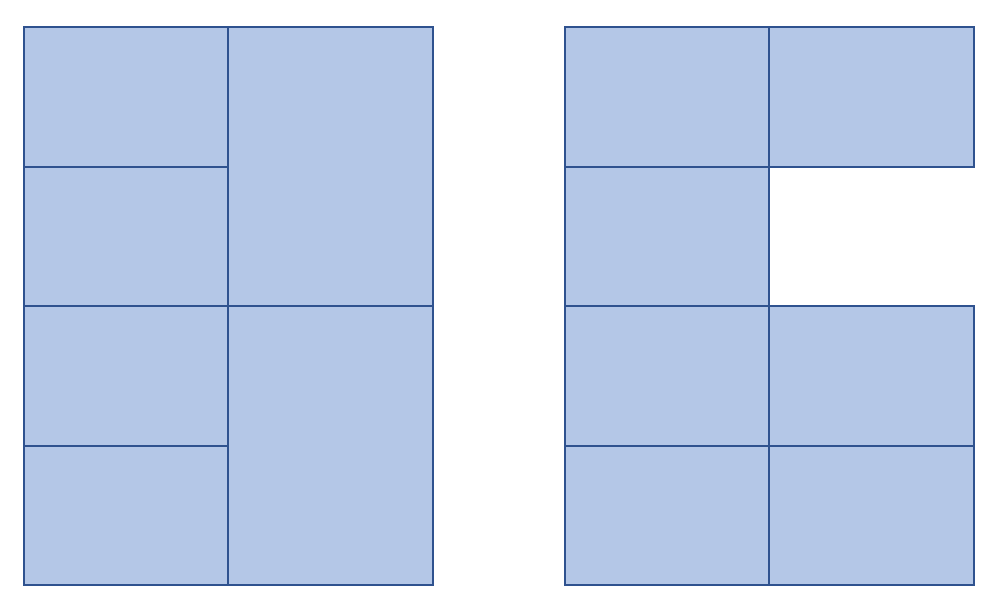
\includegraphics[width=0.8\textwidth]{graphics/structure_top.png}
	\caption[Top view of potentially problematic \ac{SLC} arrangements.]{Top view of potentially problematic \ac{SLC} arrangements.\footnotemark}
	\label{abb:structure_top}
\end{figure}
\footnotetext{Illustration by the author} 


	
	
%\blinddocument
%\input{includes/text_mit_zitaten.tex}
%\input{includes/abbildungen_und_tabellen.tex}


\chapter*{Appendix}
\addcontentsline{toc}{chapter}{Appendix}
\section*{List of appendices}
\vspace{-8em}

% vor \listofanhang müssen Einrückungen angepasst werden
\abstaendeanhangverzeichnis

\listofanhang
\clearpage
\spezialkopfzeile{Appendix} % damit in der Kopfzeile das Wort "Anhang" angezeigt wird

\anhang{Meetings}
\begin{enumerate}
	\item \label{meeting:Someone} Interview with Someone (technical lead, \ac{CV}-expert) on 29th June 2021.
	\item \label{meeting:Another Someone} Interview with Another Someone (logistics process expert) and on 30th June 2021.

	
	
\end{enumerate}	
%\anhang{Release Notes}
\anhangteil{Änderungen in Version 1.1}\label{anhang:ReleaseNotes11}
In Version 1.1 sind einige Rückmeldungen, die nach der Einführungsvorlesung am 6.2.2015 oder nach Veröffentlichung der Vorlage in Moodle eingegangen sind, berücksichtigt worden. Korrekturen sind mit \enquote{(Fix)} gekennzeichnet. 

\begin{itemize}
\item \verb|latex-vorlage.tex|
\begin{itemize}
\item (Fix) Abkürzungsverzeichnis wird vor Abbildungsverzeichnis platziert
\item (Fix) Abbildungs- und Tabellenverzeichnis in Inhaltsverzeichnis aufgenommen
\item (Fix) Quellenverzeichnis wird nun ohne Kapitelnummer dargestellt

\item eingebundene Dateien in Unterverzeichnissen \verb|includes| bzw.\ \verb|graphics|
\item Beispiel-Anhang (Datei \verb|anhang.tex|) mit Erklärungen wurde eingebunden 
\end{itemize}

\item \verb|_dhbw_praeambel.tex|
\begin{itemize}
\item (Fix) das Paket hyperref wird nach biblatex eingebunden, um ein Problem mit der Verlinkung der Fußnoten im PDF zu beheben
\item (Fix) Fußnoten  gemäß der Richtlinien fortlaufend nummeriert und nicht pro Kapitel
\item Einstellungen hinzugefügt, um Anhangsverzeichnis zu ermöglichen
\item bessere Kompatibilität zwischen KOMA-Script (scrreprt) und anderen Paketen mittels scrhack
\end{itemize}

\item \verb|_dhbw_biblatex-config.tex|
\begin{itemize}
\item (Fix) keine Abschnittsnummern für einzelne Verzeichnisse im Quellenverzeichnis
\end{itemize}

\item \verb|abbildungen_und_tabellen.tex|
\begin{itemize}
\item Erklärung, wie eine Fußnote/ein Zitat bei einer Abbildung zu erstellen ist
\end{itemize}

\item \verb|abkuerzungen.tex|
\begin{itemize}
\item Abkürzungsverzeichnis wird im Inhaltsverzeichnis aufgeführt
\end{itemize}

\item \verb|abstract.tex|, \verb|anhang.tex|, \verb|einleitung.tex| 
\begin{itemize}
\item Erklärungen im Text ergänzt
\end{itemize}

\item \verb|deckblatt.tex|
\begin{itemize}
\item Meta-Daten (Autor, Titel) für die generierte PDF-Datei lassen sich nun festlegen
\end{itemize}

\end{itemize}


\anhangteil{Änderungen in Version 1.2}\label{anhang:ReleaseNotes12}
Über das Forum in Moodle sind einige Rückmeldungen eingegangen -- vielen Dank an alle, die dazu beigetragen haben. In der Version 1.2 wurden folgende Änderungen vorgenommen, wobei Korrekturen wieder mit \enquote{(Fix)} gekennzeichnet sind: 

\begin{itemize}
\item \verb|latex-vorlage.tex| (Hauptdokument)
\begin{itemize}
\item (Fix) Zeile 19: Seitenzahlen zu Beginn mit römischen \emph{Groß}buchstaben nummeriert
\end{itemize}

\item \verb|_dhbw_praeambel.tex|
\begin{itemize}
\item Zeile 39/40: Unterstützung für \enquote{ebenda} 
\item Zeile 46--68: zweite Gliederungsebene für Anhänge ermöglicht
\item (Fix) Zeile 70--73: Abbildungen und Tabellen: Zähler fortlaufend, kein Rücksetzen zu Kapitelbeginn (Paket \verb|chngcntr| anstelle von Paket \verb|remreset|)
\end{itemize}

\item \verb|_dhbw_biblatex-config.tex|
\begin{itemize}
\item (Fix) bei Quellen mit Herausgeber, aber ohne Autor wird der Name des Herausgebers im Verzeichnis fett gedruckt
\item Unterstützung für \enquote{ebenda} 
\end{itemize}

\item \verb|abkuerzungen.tex|
\begin{itemize}
\item Bemerkungen zur fortgeschrittenen Nutzung des \verb|acronym|-Pakets eingefügt 
\end{itemize}

\item \verb|einleitung.tex|
\begin{itemize}
\item Abschnitt 1.3 zu Einstellungen ergänzt
\item Abschnitt 1.5 zu Fehlerbehebungen eingefügt 
\end{itemize}

\item \verb|text-mit-zitaten.tex|
\begin{itemize}
\item Abschnitt 3.1 eingefügt, Erläuterungen zum Zitieren mit \enquote{vgl.} und \enquote{ebenda}. 
\item Abschnitt 3.2: Beispiele ergänzt
\item Hinweis zu Jahreszahlen bei Online-Quellen
\end{itemize}

\item \verb|anhang.tex|
\begin{itemize}
\item Erläuterungen zur zweiten Gliederungsebene
\end{itemize}

\item \verb|literatur-datenbank.bib|
\begin{itemize}
\item weitere Beispiele für Quellen
\end{itemize}

\end{itemize}

\anhangteil{Änderungen in Version 1.3}\label{anhang:ReleaseNotes13}
Durch die ab 1/2016 geltenden Änderungen der Zitierrichtlinien des Studiengangs waren einige kleinere Anpassungen der Vorlage erforderlich, die nachfolgend beschrieben sind. Bei dieser Gelegenheit ebenfalls erfolgte Korrekturen sind wieder mit \enquote{(Fix)} gekennzeichnet:

\begin{itemize}
\item \verb|latex-vorlage.tex| (Hauptdokument)
\begin{itemize}
\item Hinweis auf Option doppelseitiger Druck entfernt
\item Schriftgröße der Kapitelüberschriften verkleinert
\item (Fix) Kopf- und Fußzeilen werden nun korrekt angezeigt für erste Seite eines Kapitels und auch  Quellenverzeichnisse
\end{itemize}

\item \verb|_dhbw_praeambel.tex|
\begin{itemize}
\item Angabe des unteren Rands für Seitenzahl, da diese nun unten rechts steht
\item Unterstützung für \enquote{ebenda} entfernt
\item (Fix) Präfixe wie \enquote{von} im Namen eines Autors werden berücksichtigt
\item Anpassung der Abstände bei Kapitelüberschriften
\item Kopf- und Fußzeile für Verzeichnisse nun in \verb|_dhbw_kopfzeilen.tex| definiert 
\end{itemize}


\item \verb|deckblatt.tex|
\begin{itemize}
\item Schriftgröße des Titels vergrößert
\item Befehl \verb|\typMeinerArbeit| eingeführt, um Typ auszuwählen
\item Festlegung des Themas (für ehrenwörtliche Erklärung) mit Befehl \verb|\themaMeinerArbeit|
\item Darstellung der Angabe des Betreuers in der Ausbildungsstätte angepasst
\item Formulierung des Sperrvermerks angepasst  
\end{itemize}

\item \verb|_dhbw_erklaerung.tex|
\begin{itemize}
\item Formulierung angepasst an geänderte Prüfungsordnung
\item Typ und Thema der Arbeit werden automatisch eingefügt
\end{itemize}

\item \verb|_dhbw_kopfzeilen.tex|
\begin{itemize}
\item Seitennummern stehen jetzt unten rechts
\item (Fix) Kopf- und Fußzeile werden nun korrekt angezeigt in Verzeichnissen und dem Anhang
\end{itemize}

\item \verb|_dhbw_biblatex-config.tex|
\begin{itemize}
\item Anpassung des Zitierstils auf die ab 1/2016 geltenden Regelungen  
\item Vorkehrungen für Eindeutigkeit (Hinzufügen abgekürzter oder nötigenfalls ausgeschriebener Vorname) bei Übereinstimmung von Name und Jahreszahl 
\end{itemize}

\item \verb|einleitung.tex|
\begin{itemize}
\item Abschnitt 1.3 zu Einstellungen grundlegend überarbeitet
\item Abschnitt 1.5.2 zur Kontrolle der Seitenränder eingefügt 
\end{itemize}

\item \verb|text-mit-zitaten.tex|
\begin{itemize}
\item Abschnitt 3.1: Hinweise zu \enquote{ebenda} entfernt
\item Abschnitt 3.2: Beispiele zur Eindeutigkeit des Zitats ergänzt
\item Abschnitt 3.3: Hinweise für E-Journals/E-Books ergänzt 
\end{itemize}

\item \verb|anhang.tex|
\begin{itemize}
\item (Fix) Befehl \verb|\spezialkopfzeile| aufgenommen, damit in Kopfzeile das Wort \enquote{Anhang} angezeigt wird 
\item diese Release Notes wurden in eine eigene Datei verschoben
\end{itemize}

\item \verb|release_notes.tex|
\begin{itemize}
\item s.o.
\end{itemize}


\item \verb|literatur-datenbank.bib|
\begin{itemize}
\item weitere Beispiele für Quellen
\end{itemize}
\end{itemize}

\anhangteil{Änderungen in Version 1.4}\label{anhang:ReleaseNotes14}
Durch nicht abwärtskompatible Änderungen beim Versionswechsel von Biblatex 3.2 zu 3.3 sind einige Änderungen notwendig geworden.\footnote{Diese basieren auf Vorschlägen von Yannik Ehlert -- vielen Dank dafür!}
Die vorliegende Version 1.4 wurde erfolgreich mit MikTeX gestestet (portable Version 2.9.6361 vom 3.6.2017, unter Verwendung von Biblatex 3.7).

\begin{itemize}
\item \verb|_dhbw_biblatex-config.tex|
\begin{itemize}
\item Anpassung der \verb|\usebibmacro|-Befehle
\end{itemize}

\item \verb|_dhbw_authoryear.bbx|
\begin{itemize}
\item  Änderung von \verb|\printdateextralabel| zu \verb|\printlabeldateextra|
\end{itemize}
\end{itemize}

\anhangteil{Änderungen in Version 1.5}\label{anhang:ReleaseNotes15}
Für den Test dieser Version auf einem Windows-System wurde wieder die portable Version von MiKTeX (2.9.6521 vom 10.11.2017) verwendet.\footnote{\url{http://miktex.org/portable}} Da in diesem Paket leider die Versionen von Biblatex (3.10) und Biber (2.7) inkompatibel sind, ist es erforderlich, die Datei \verb|biber.exe| im Verzeichnis \verb|texmfs\install\miktex\bin\| durch die aktuelle Version 2.10 vom 20.12.2017\footnote{\url{https://sourceforge.net/projects/biblatex-biber/files/biblatex-biber/current/binaries/Windows/}} zu ersetzen. Im Editor TeXworks verwendet man dann zum Übersetzen des \LaTeX-Sourcecodes Typeset/pdfLaTeX bzw.\ Typeset/Biber.

Korrekturen sind wieder mit \enquote{(Fix)} gekennzeichnet.

\begin{itemize}
\item \verb|latex-vorlage.tex| (Hauptdokument)
\begin{itemize}
\item Nach der Änderung der Zitierrichtlinien gibt es nun kein separates Verzeichnis mehr für Internet- und Intranetquellen.
\item Option \verb|notkeyword=ausblenden| bei \verb|\printbibligraphy| sorgt dafür, dass Sekundärliteratur korrekt zitiert wird.
\end{itemize}

\item \verb|_dhbw_praembel.tex|
\begin{itemize}
\item (Fix) Die Bezeichnung geschachtelter Anhänge wurde auf das in den Zitierrichtlinien geforderte Format \enquote{Anhang 2/1} angepasst (Befehl \verb|\anhangteil|).
\end{itemize}

\item \verb|einleitung.tex|
\begin{itemize}
\item Hinweis zum Ausblenden der farbigen Links im PDF hinzugefügt
\end{itemize}

\item \verb|text-mit-zitaten.tex|
\begin{itemize}
\item Abschnitt 3.4 aktualisiert nach Wegfall des separaten Verzeichnisses für Internet- und Intranetquellen
\item Abschnitt zum Zitieren von Sekundärliteratur hinzugefügt
\end{itemize}

\end{itemize}


\anhangteil{Änderungen in Version 1.6}\label{anhang:ReleaseNotes16}
Diese Version wurde auf einem Windows-System erfolgreich mit der portablen Version von MiKTeX (2.9.6621 vom 18.02.2018) getestet.\footnote{Vielen Dank an Florian Eichin für seine wertvollen Anmerkungen.}

Korrekturen sind wieder mit \enquote{(Fix)} gekennzeichnet.

\newpage

\begin{itemize}
\item \verb|latex-vorlage.tex| (Hauptdokument)
\begin{itemize}
\item (Fix) An einer Stelle gab es in Version 1.5 (Internetquellen nicht mehr separat) noch ein Überbleibsel von Version 1.4 (Internetquellen separat), dies wurde korrigiert.
\item (Fix) Im Inhaltsverzeichnis war die Verlinkung des Abbildungs- und Tabellenverzeich\-nisses nicht ganz korrekt.
\item Mit den Befehlen \verb|\literaturverzeichnis| bzw.\ \verb|\literaturUndQuellenverzeichnis| kann bequem die Erstellung der Quellenverzeichnisse gesteuert werden, abhängig davon, ob es ein Gesprächsverzeichnis gibt oder nicht.
 
\end{itemize}

\item \verb|_dhbw_praembel.tex|
\begin{itemize}
\item Einrückungen für Abbildungs-, Tabellen- und Anhangverzeichnis angepasst
\item Abkürzungen \enquote{Abb.} und \enquote{Tab.} für Abbildungen bzw.\ Tabellen
\end{itemize}

\item \verb|_dhbw_biblatex-config.tex|
\begin{itemize}
\item Befehle \verb|\literaturverzeichnis| und \verb|\literaturUndGespraechsverzeichnis| definiert
\item Befehl \verb|\footcitePrimaerSekundaer| definiert
\end{itemize}

\item \verb|_dhbw_erklaerung.tex|
\begin{itemize}
\item Eintrag als \enquote{Erklärung} (statt \enquote{Ehrenwörtliche Erklärung}) ins Inhaltsverzeichnis
\end{itemize}

\item \verb|einleitung.tex|
\begin{itemize}
\item Bezeichnung \enquote{Erklärung} statt \enquote{Ehrenwörtliche Erklärung}
\item Erläuterung von \verb|\literaturverzeichnis| und \verb|\literaturUndGespraechsverzeichnis|
\item Hinweis auf Notwendigkeit von Updates bei MikTeX Portable
\end{itemize}

\item \verb|text_mit_zitaten.tex|
\begin{itemize}
\item Erläuterungen zu Befehl \verb|\footcitePrimaerSekundaer| ergänzt
\end{itemize}

\item \verb|anhang.tex|
\begin{itemize}
\item Befehl \verb|\abstaendeanhangverzeichnis| für Anpassung Einrückung ergänzt
\end{itemize}

\item \verb|literatur-datenbank.bib|
\begin{itemize}
\item Eintrag ergänzt
\end{itemize}

\end{itemize}

\anhangteil{Änderungen in Version 1.7}\label{anhang:ReleaseNotes17}
Diese Version wurde auf einem Windows-System erfolgreich mit der portablen Version von MiKTeX (2.9.6942 vom 04.01.2019) getestet.

Korrekturen sind wieder mit \enquote{(Fix)} gekennzeichnet.

\begin{itemize}
\item \verb|_dhbw-authoryear.bbx|
\begin{itemize}
\item Da \verb|labeldate| in Biblatex nicht mehr unterstützt wird, erfolgte eine Umbenennung in 
\verb|labeldateparts|.\footnote{vgl.\ \url{https://github.com/semprag/biblatex-sp-unified/issues/23}}
\end{itemize}

\item \verb|_dhbw_biblatex-config.tex|
\begin{itemize}
\item (Fix) Es wurde das Problem behoben, dass im Literaturverzeichnis bei bestimmten Eintragstypen der Titel in Anführungszeichen steht.\footnote{Danke an Florian Eichin für seinen Hinweis.}
\end{itemize}

\end{itemize}


\anhangteil{Änderungen in Version 1.8}\label{anhang:ReleaseNotes18}
Diese Version wurde auf einem Windows-System erfolgreich mit der portablen Version von MiKTeX (2.9.6942 vom 04.01.2019) getestet.

Die Aktualisierungen in der Vorlage spiegeln zum Einen die Änderungen in den Zitierrichtlinien wieder. Zum Anderen wurden einige studentische Vorschläge aufgegriffen, um die Nutzung der Vorlage zu erleichtern.\footnote{Danke an Bjarne Koll, Tobias Schwarz und Lars Ungerathen für ihre Anregungen.} 

\begin{itemize}

\item \verb|latex_vorlage.tex| (Hauptdokument)
\begin{itemize}
\item Es wird nun davon ausgegangen, dass die zur Vorlage gehörenden Dateien in einem eigenen Verzeichnis (\verb|template|) liegen.
\item Stellenweise wurden Erläuterungen als Kommentare hinzugefügt.
\end{itemize}

\item \verb|_dhbw_biblatex-config.tex|
\begin{itemize}
\item Code, der mehrere Quellenverzeichnisse unterstützt, wurde entfernt.
\item Ein zu großer Abstand nach Zitaten von Sekundärliteratur wurde korrigiert. 
\end{itemize}

\item \verb|_dhbw_erklaerung.bbx|
\begin{itemize}
\item Gemäß der Anforderung in den Zitierrichtlinien wird die Erklärung nicht ins Inhaltsverzeichnis aufgenommen und nicht mit einer Seitenzahl versehen. 
\end{itemize}

\pagebreak
\item \verb|_dhbw_praeambel.bbx|
\begin{itemize}
\item Gemäß der Anforderung in den Zitierrichtlinien werden im Literaturverzeichnis alle Autor/innen eines Werks angegeben.
\end{itemize}

\item \verb|abstract.tex|
\begin{itemize}
\item Hinweis auf \LaTeX-Spickzettel hinzugefügt.
\end{itemize}

\item \verb|deckblatt.tex|
\begin{itemize}
\item Vorname, Name, Titel der Arbeit sind nur zu Beginn einzutragen und werden dann an den entsprechenden Stellen automatisch ergänzt.
\item Hervorhebung, dass Angaben zum Unternehmen sowie den Betreuer/innen zu ergänzen sind. 
\item Wortlaut des Vertraulichkeitsvermerks wurde an die aktuelle Fassung in der Studien- und Prüfungsordnung angepasst. 
\end{itemize}

\item \verb|einleitung.tex|
\begin{itemize}
\item Ein eigenständiges Gesprächsverzeichnis als Teil des Quellenverzeichnisses ist in den Zitierrichtlinien nicht mehr vorgesehen, die entsprechenden Hinweise wurden entfernt.
\item Ein alter Hinweis auf die Darstellung von Links im Verzeichnis der Internetquellen wurde entfernt, da es ein solches eigenständiges Verzeichnis nicht mehr gibt. 
\end{itemize}

\item \verb|text_mit_zitaten.tex|
\begin{itemize}
\item Es wird nun erläutert, wie zwei Quellenangaben unmittelbar nebeneinander dargestellt werden können.
\item Erklärungen, die von mehreren Quellenverzeichnissen ausgegangen sind, wurden entfernt.
\end{itemize}

\item \verb|literatur-datenbank.bib|
\begin{itemize}
\item Gespräch wurde entfernt, da dieses nicht mehr im Quellenverzeichnis aufgeführt werden soll.
\end{itemize}

\end{itemize}
%%% Ende des eigentlichen Inhalts %%%


%%% Quellenverzeichnisse (keine Anpassung nötig) %%%
\clearpage
\literaturverzeichnis

%%% Ende Quellenverzeichnisse %%%


%%% Erklärung (keine Anpassungen nötig) %%%
% steht ganz am Ende des Dokuments
\cleardoublepage
\clearpage

\thispagestyle{empty}

{\LARGE\textsf{\textbf{Declaration}}\bigskip}

% \typMeinerArbeit und \themaMeinerArbeit werden in deckblatt.tex definiert


I hereby insure that I have personally authored my project work with the topic: \emph{\themaMeinerArbeit} and have used no sources and aids other than those indicated. I also
insure that the submitted electronic version corresponds to the printed version. 

\vspace{3cm}

\begin{center}
\begin{tabular}{ccc}
(place, date) & \hspace{0.3\linewidth} & (signature)
\end{tabular}
\end{center}
\end{document}